\documentclass[a4paper,11pt,oneside,openany]{jsbook}
\usepackage{myjlabthesisstyle}
\daigaku{青山学院大学}
\gakubu{社会情報学部}
\gakka{社会情報学科}
\syubetsu{卒業論文}
\labname{宮治研究室}
\chiefexaminer{宮治~~裕~~教授}

%%%%%%%%%%%%%%%%%%%%%%%%%%%%%%%%%%%%%%%
% ここから先「ここまで個人設定」の範囲に
% 各自の固有の情報を記入して下さい
%%%%%%%%%%%%%%%%%%%%%%%%%%%%%%%%%%%%%%%
\nendo{2021年度}
\teisyutsu{2022年~~1月}
\snum{18118047}
\jname{黒川~~皇輝}
\thesistitle{PLSAとMAP推定を用いた日本語歌詞の印象推定手法の評価} %タイトルを記入
%\thesissubtitle{\LaTeX の利用} %サブタイトルを記入 ない場合はコメントアウト
%\SUBTtrue %サブタイトル有りの場合 ない場合は,コメントアウト
\SUBTfalse %サブタイトル無しの場合 有る場合は,コメントアウト
%%%%%%%%%% ここまで個人設定 %%%%%%%%%%%%%%
\begin{document}

\chapter{歌詞の印象推定}
本研究で行った歌詞の印象推定法について説明する.最初に研究で用いた分析手法について述べたのちに,分析手法を活用した歌詞の印象推定手法について述べる.その後,分析結果を記述する.
\section{分析手法}
この節では歌詞印象推定手法で用いた分析手法について紹介する.
\subsection{MAP推定}
MAP推定とは事前知識に基づいて未知のデータを点推定する手法である.
θを尤度,Dを事前知識とすると,ベイズの定理に基づき次の式(3.1)で表せる.
\begin{equation}
\begin{split}
\rm{argmax_{θ}P(θ|D)}&\rm{=argmax_θ\frac{P(D|θ)P(θ)}{P(D)}}\\
&\rm{=argmax_{θ}P(D|θ)P(θ)}
\end{split}
\end{equation}
ここで分母のP(D)は尤度θと関係がないので無視する.P(D\verb+|+θ)は尤度関数,P(θ)は事前分布,P(θ\verb+|+D)は事後分布と呼ぶ.
事前分布P(θ)は複雑な計算を要する.そのため,それを回避するために事前分布の代わりに共役事前分布を用いて推定をする.共役事前分布とは尤度をかけて事後分布を求めるとその関数の形が同じになる事前分布のことである.
事後分布が最大となる尤度θを算出するのがMAP推定である.

本研究ではカテゴリカル分布に基づくMAP推定をする.
したがって事前知識Dはカテゴリカル分布に従うN個の離散値データ$\rm{D=\{d_1,d_2,...d_N\}}$と定義する.
尤度関数はカテゴリカル分布の確立質量関数で表せるので式(3.2)となる.
\begin{equation}
\begin{split}
\rm{P(D|θ)=\prod^N_{n=1}Cat(d_n|θ)}
\end{split}
\end{equation}
カテゴリカル分布の共役事前分布はディリクレ分布であるため事前分布を式(3.3)で表す.ディリクレ分布はハイパーパラメータαが大きくなるにつれて分散が小さくなる特性を持つ.
ハイパーパラメータαは対応する事象dの観測数の初期値を意味する.αを全て1とした場合,ディリクレ分布は一様な無情報事前分布となり,事後分布は尤度関数であるカテゴリカル分布と同じ分布になる.
\begin{equation}
\begin{split}
\rm{P(θ)\propto{Dir(θ;\alpha)}}
\end{split}
\end{equation}
式(3.2)と式(3.3)を式(3.1)に当てはめると事後分布は式(3.4)のように表せる.
\begin{equation}
\begin{split}
\rm{P(θ|D)\propto\{\prod^N_{n=1}Cat(d_n|θ)\}Dir(θ;\alpha)}
\end{split}
\end{equation}
式(3.4)の両辺に対数をとった式(3.5)を示す.ここで$\rm{d_{n,k}}$はK次元ベクトル$\rm{d_n}$のk番目の要素を指し示す.$\mathbb{C}$は不定定数である.
\begin{equation}
\begin{split}
\rm{\log P(θ|D)}&\rm{\propto\sum^N_{n=1}\log Cat(d_n|θ)+\log Dir(θ;\alpha)+\mathbb{C}}\\
&\rm{=\sum^K_{k=1}(\sum^N_{n=1}d_{n,k}+\alpha_{n,k}-1)\log θ_k+\mathbb{C}}
\end{split}
\end{equation}
このまま偏微分しても極値を得ることはできないのでラグランジュの未定乗数法を使用する.ラグランジュ関数は式(3.6)である.
\begin{equation}
\begin{split}
\rm{L=\log P(θ|D)+\lambda(\sum^K_{k=1}θ_k-1)}
\end{split}
\end{equation}
ラグランジュ関数Lを$\rm{θ_k}$で偏微分して0となる極値を求めるとMAP推定値$\rm{{\hat\mu}_{map,k}}$が得られる.
\begin{equation}
\begin{split}
\rm{{\hat\mu}_{map,k}=\frac{\alpha_k-1+θ_k}{1-K+\sum^K_{j=1}\alpha_j}}
\end{split}
\end{equation}
\subsection{PLSA}
PLSA[12]とは次元圧縮手法の一種であり,情報検索の分野で膨大な文書データを分類するために研究された手法である.
PLSAは文書dとその文書中に出現する単語wの間に共通のトピックと呼ぶ潜在意味クラスzが存在することを想定として,潜在意味クラスzを確率的に推定する手法である.
そして,文書dと単語wの共起確率P(d,w)を潜在意味クラスzを用いてモデル化する.zでモデル化したP(d,w)の式を式(3.8)にグラフィカルモデルを図1に示す.
\begin{equation}
\begin{split}
\rm{P(d,w)=\sum_zP(z)P(d|z)P(w|z)}
\end{split}
\end{equation}

\begin{figure}[h]
  \centering
  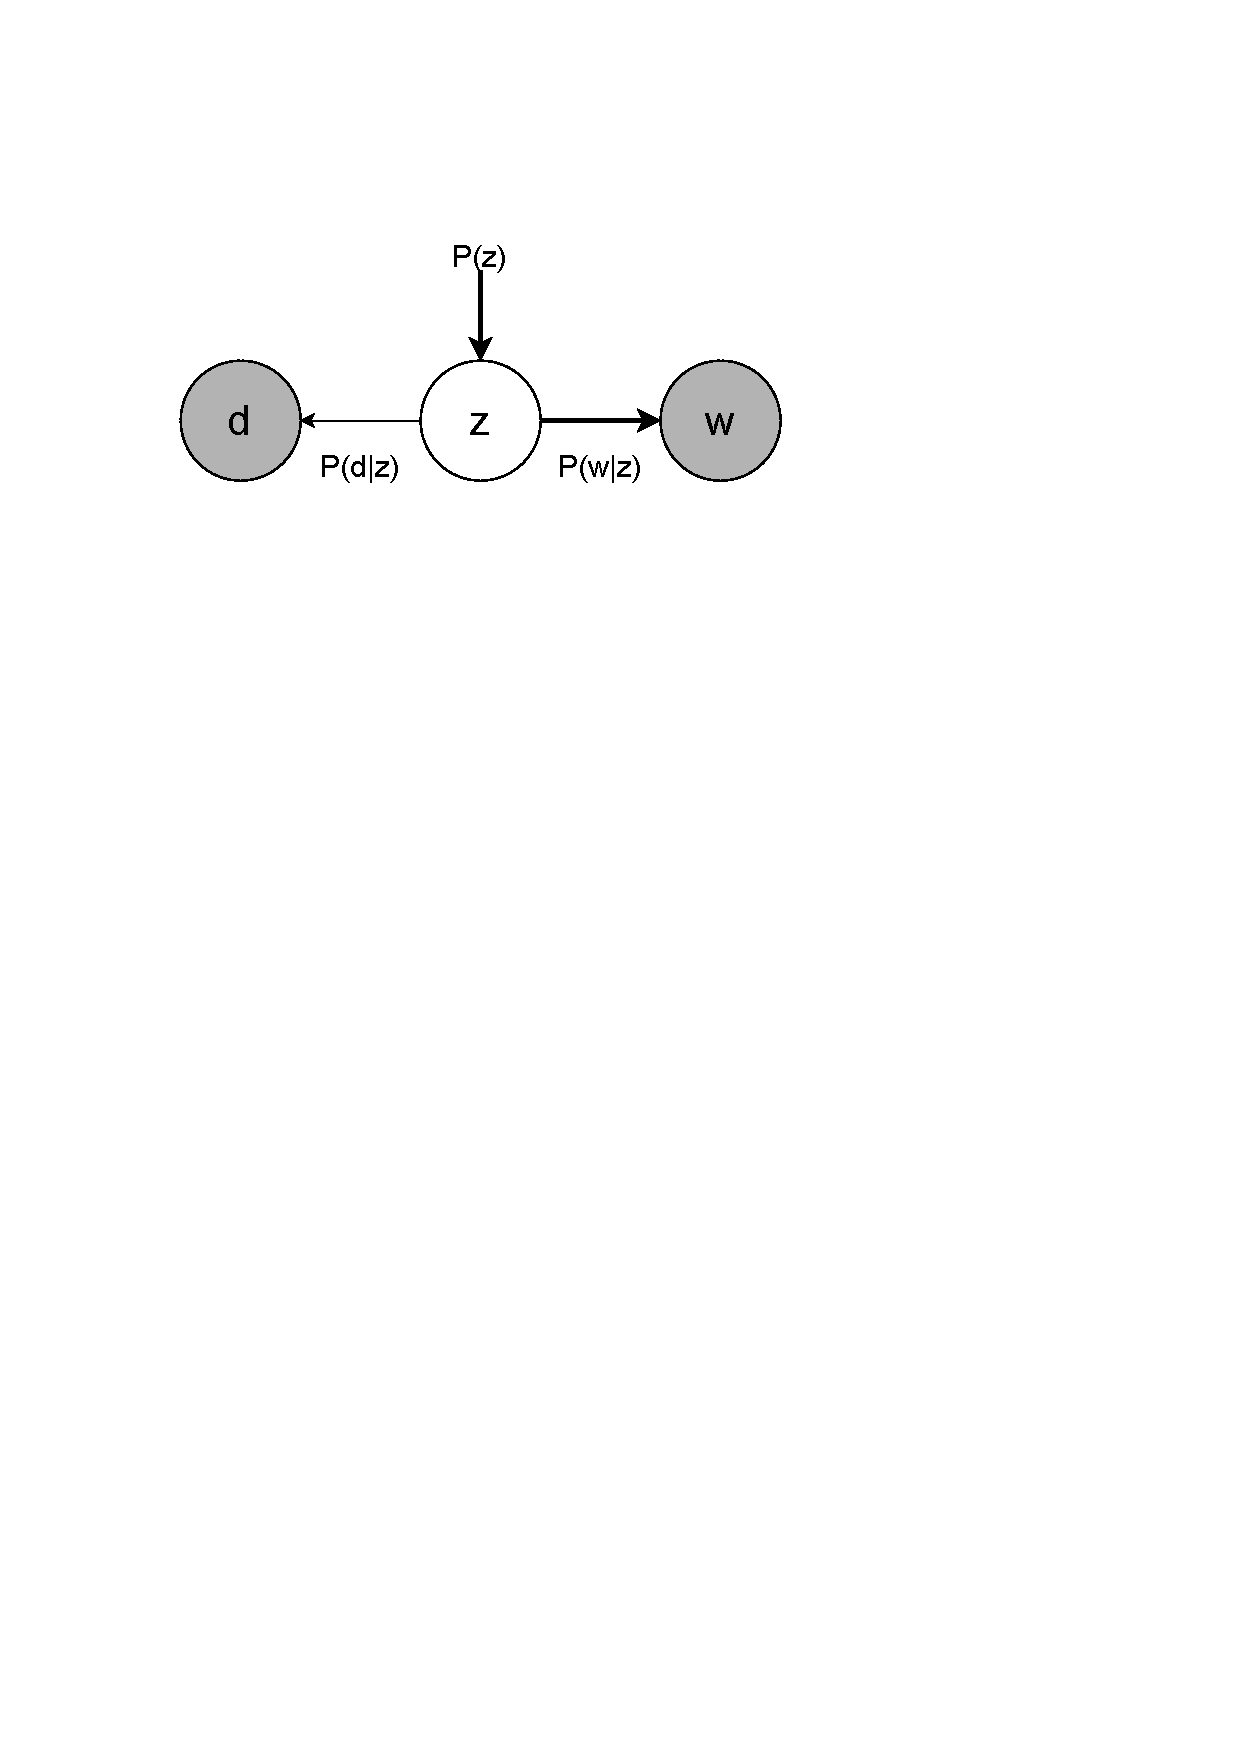
\includegraphics[width=12cm]{PLSA_graphical.pdf}
  \vspace{-1mm}
  \caption{PLSAグラフィカルモデル}
  \label{fig:vkall}
  \vspace{5mm}
\end{figure}
文書dと単語wの同時出現頻度をN(d,w)とすると,対数尤度関数logLは式(3.9)として示せる.
\begin{equation}
\begin{split}
\rm{\log L= \sum_d\sum_wN(d,w)\log(P(d,w))}
\end{split}
\end{equation}
この対数尤度関数logLを最大にする確率変数P(z),P(d\verb+|+z),P(w\verb+|+z)をEMアルゴリズムによって推定する.なお推定する確率変数をモデルパラメータと呼ぶ.EMアルゴリズムとは混合分布モデルのパラメータ推定に利用できる学習アルゴリズムである.
zの確率分布P(z\verb+|+d,w)を予測するE(expectation)ステップと対数尤度関数の最大化をするM(maximization)ステップに計算ステップが分かれている.それぞれのステップで行われる計算の説明を順番に述べる.
式(3.10)はEステップの式である.初期値であるP(z),P(d\verb+|+z),P(w\verb+|+z)は絶対値が1以下のランダムな自然数に決定され,zの確率分布P(z\verb+|+d,w)を予測する.

\begin{equation}
\rm{P(z|d,w)=\frac{P(d|z)P(w|z)P(z)}{\sum_zP(d|z)P(w|z)P(z)}}
\end{equation}
式(3.11)(3.12)(3.13)はMステップの式であり,それぞれの式でモデルパラメータを求めている.

\begin{equation}
\rm{P(d|z)=\frac{\sum_wN(d,w)P(z|d,w)}{\sum_d\sum_wN(d,w)P(z|d,w)}}
\end{equation}

\begin{equation}
\rm{P(w|z)=\frac{\sum_dN(d,w)P(z|d,w)}{\sum_d\sum_wN(d,w)P(z|d,w)}}
\end{equation}

\begin{equation}
\rm{P(z)=\frac{\sum_d\sum_wN(d,w)P(z|d,w)}{\sum_d\sum_w\sum_zN(d,w)P(z|d,w)}}
\end{equation}
求めたモデルパラメータを式(3.2)に当てはめて式(3.3)の対数尤度関数の値を求める.対数尤度関数の値を最大化するまでEステップとMステップを交互に繰り返し,最適なモデルパラメータを求める.

\subsection{日本語版ANEW拡張データセット}
本間らが開発した日本語版ANEWの単語の類義語と同義語をWordNet[14]を用いて探索する.発見した単語に類義語元の単語が持つArousalとValenceの値を与えることで,日本語版ANEWを14,232語に拡張した単語データセットを日本語版ANEW拡張データセットとする.
日本語版ANEW拡張データセットの構成は後述するA+V+平面に5,581語,A+V-平面に2,681語,A-V-平面に3,456語,A-V+平面に2,493語である.
\newpage
\section{歌詞の印象推定手法}
この節では歌詞の印象推定手法について紹介する.

\subsection{印象の定義}
本稿で推定する印象とはRussellのAV平面上で表現する.AV平面は縦軸にArousalを,横軸にValenceを取る2次元平面である.Arousal軸は正の方向に興奮を,負の方向に弛緩を表す.そして,Valence軸は正の方向に快を,負の方向に不快を表す.
AV平面の4象限は大まかに喜怒哀楽の印象を表す.第1象限は喜びや幸福,興奮,驚きといった喜の感情グループを表す.第2印象は怒りや恐れ,嫌悪といった怒の感情グループを表す.第3章限は退屈や悲しみ,
憂鬱といった哀の感情グループを表す.第4象限は満足や穏やか,くつろぎといった楽の感情グループを表す.AV平面に歌詞データをプロットし,データが存在する象限から歌詞データを4つのグループの印象にクラスタリングする.

\subsection{歌詞データの収集}
歌詞データの収集はUta-Net\footnote{https://www.uta-net.com/}から人気のアーティストの曲を6,813曲収集した.本研究では6,813曲から3,000曲を無作為に選んだ.

\subsection{歌詞データの整形}
収集した歌詞データの中に一部英語が入っていたので,英語の歌詞を削除した.そして歌詞データを歌詞のフレーズごとに分解した.形態素解析器MeCabを用いて各フレーズから名詞・形容詞・動詞を抜き出した.歌詞から抜き出した単語の総数は109450語である.

\subsection{歌詞印象推定}
確率的潜在意味解析(PLSA)を利用する.歌詞のフレーズを文書dとし,フレーズ中に出現する単語を単語wと定義してモデルパラメータを推定した.
P(w\verb+|+z)はトピックから単語が観測される確率であるため,この確率の高い単語がトピックを表現する.
歌詞の印象を推定するためには潜在的なトピックzを印象に制限する必要がある.通常のPLSAは文書と単語の共起確率に着目して,潜在的なトピックを推定する手法であるため,必ず潜在的なトピックが印象を表現するとは限らない.
よって,日本語版ANEW拡張データセットを事前知識として使用し,モデルパラメータをMAP推定することで潜在的なトピックにAV平面の各象限を表現する.
具体的に潜在的なトピックzを次の式(3.14)のようにAV平面の各印象として定義する.
\begin{equation}
\rm{z\in\{A+V+,A+V-,A-V-,A-V+\}}
\end{equation}
モデルパラメータP(w\verb+|+z)の対数事前分布を共役事前分布を用いて式(3.15)に定義する.kは出現する単語の集合を表す.
\begin{equation}
\rm{log P(w_k|z)\propto\sum_k\sum_z(\alpha_{w_k,z}-1)\log P(w_k|z)}
\end{equation}
共役事前分布のハイパーパラメータαは日本語版ANEW拡張データセットに含まれる単語で該当の象限に位置する場合のみ原点からの距離を入力する.それ以外の場合無情報事前分布を与える.
ラグランジュの未定乗数法を使用して対数尤度関数と対数事前分布よりMAP推定値を求める
MAP推定値は式(3.16)で表す.NはMAP推定前のP(w\verb+|+z)の和である.
\begin{equation}
\rm{P(w_k|z)_{map}=\frac{\alpha_{w_k,z}-1+p(w_k|z)}{1-K+\sum_k\alpha_{w_k,z}}}
\end{equation}
P(z)とP(d\verb+|+z)の推定には無情報事前分布を与えた.
各印象ごとに単語wが出現する確率P(w\verb+|+z)をMAP推定した.ベイズの定理よりP(z\verb+|+w)は式(3.17)で求められる.
\begin{equation}
\rm{P(z|w_k)=\frac{P(w_k|z)_{map}P(z)}{P(w_k)}}
\end{equation}
P(w)は単語が出現する確率である.ある単語の出現数を全ての単語の出現数で割ると求まる.
各フレーズdのArousalとValenceの値は求めたP(z\verb+|+w)を用いて求めた各単語wのArousalとValenceの値を合計.正規化して求める.式は(3.18,3.19)である.Kはあるフレーズに出現する単語数である.
\begin{equation}
\rm{V=\frac{1}{K} \sum_{k=1}^{K}\left(\left(P\left(\mathrm{~A}+\mathrm{V}+\mid w_{k}\right)+P\left(\mathrm{~A}-\mathrm{V}+\mid w_{k}\right)\right)-\left(P\left(\mathrm{~A}+\mathrm{V}-\mid w_{k}\right)+P\left(\mathrm{~A}-\mathrm{V}-\mid w_{k}\right)\right)\right)}
\end{equation}
\begin{equation}
\rm{A=\frac{1}{K} \sum_{k=1}^{K}\left(\left(P\left(\mathrm{~A}+\mathrm{V}+\mid w_{k}\right)+P\left(\mathrm{~A}+\mathrm{V}-\mid w_{k}\right)\right)-\left(P\left(\mathrm{~A}-\mathrm{V};\mid w_{k}\right)+P\left(\mathrm{~A}-\mathrm{V}-\mid w_{k}\right)\right)\right)}
\end{equation}
以上で歌詞中のフレーズごとに感情価を求める.
\newpage
\section{AV平面にプロット}
この節では歌詞をAV平面上にプロットした結果について記述する.

\subsection{楽曲}
楽曲に登場する歌詞のフレーズのAV値の平均を歌詞のAV値とした.図3.2はAV平面に楽曲をプロットした図である.
\begin{figure}[h]
    \centering
    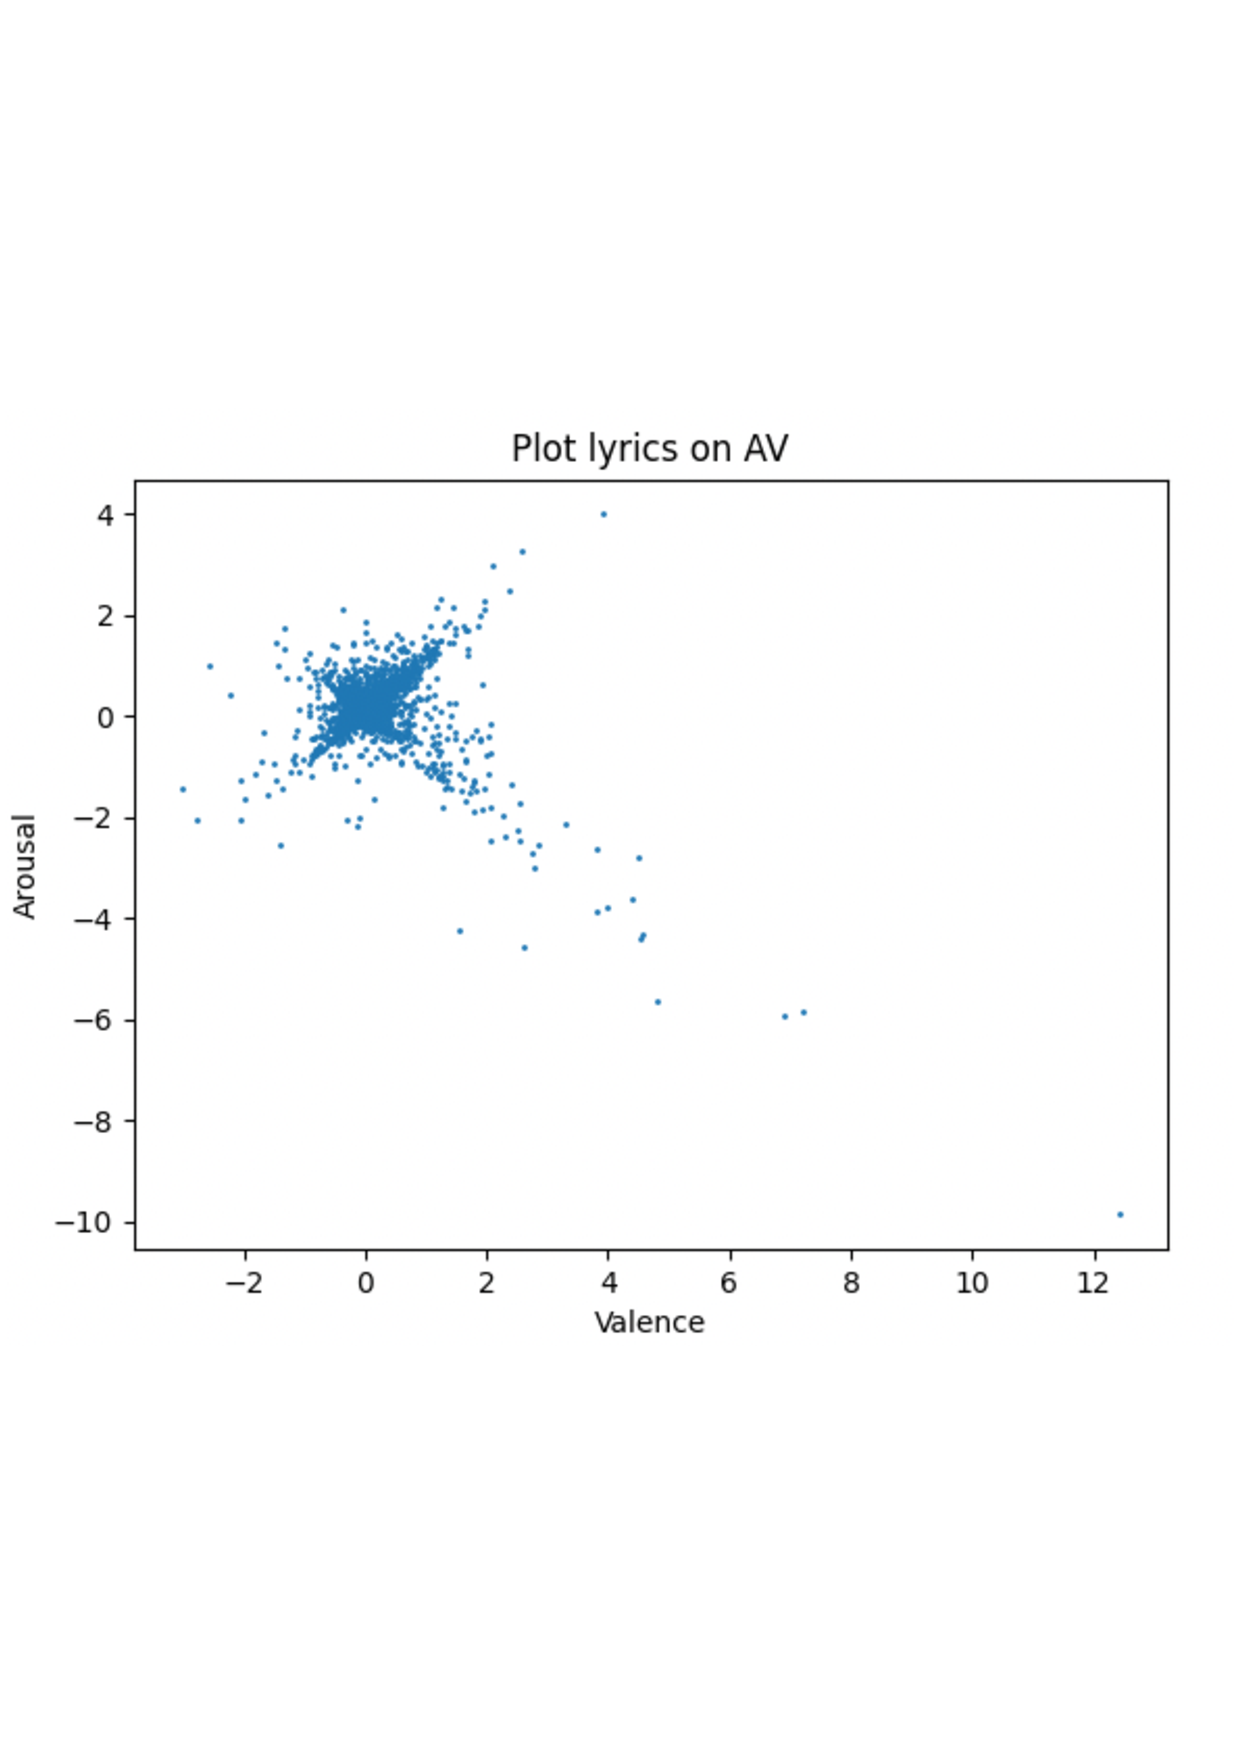
\includegraphics[width=12cm]{lyrics_AV.pdf}
    \vspace{0mm}
    \caption{歌詞 AV平面}
    \label{fig:vkall}
    \vspace{5mm}
\end{figure}

各印象ごとに歌詞を分類して,ward法で原点からの距離に基づいて3グループにクラスタリングした.
薄い肌色でプロットされている原点から一番近いグループを第1グループ.赤紫色でプロットされている原点から2番目に近いグループを第2グループ.黒色でプロットされている原点からもっとも遠いグループを第3グループとする.
\newpage
第1象限のプロット図は図3.3である.
\begin{figure}[H]
  \centering
  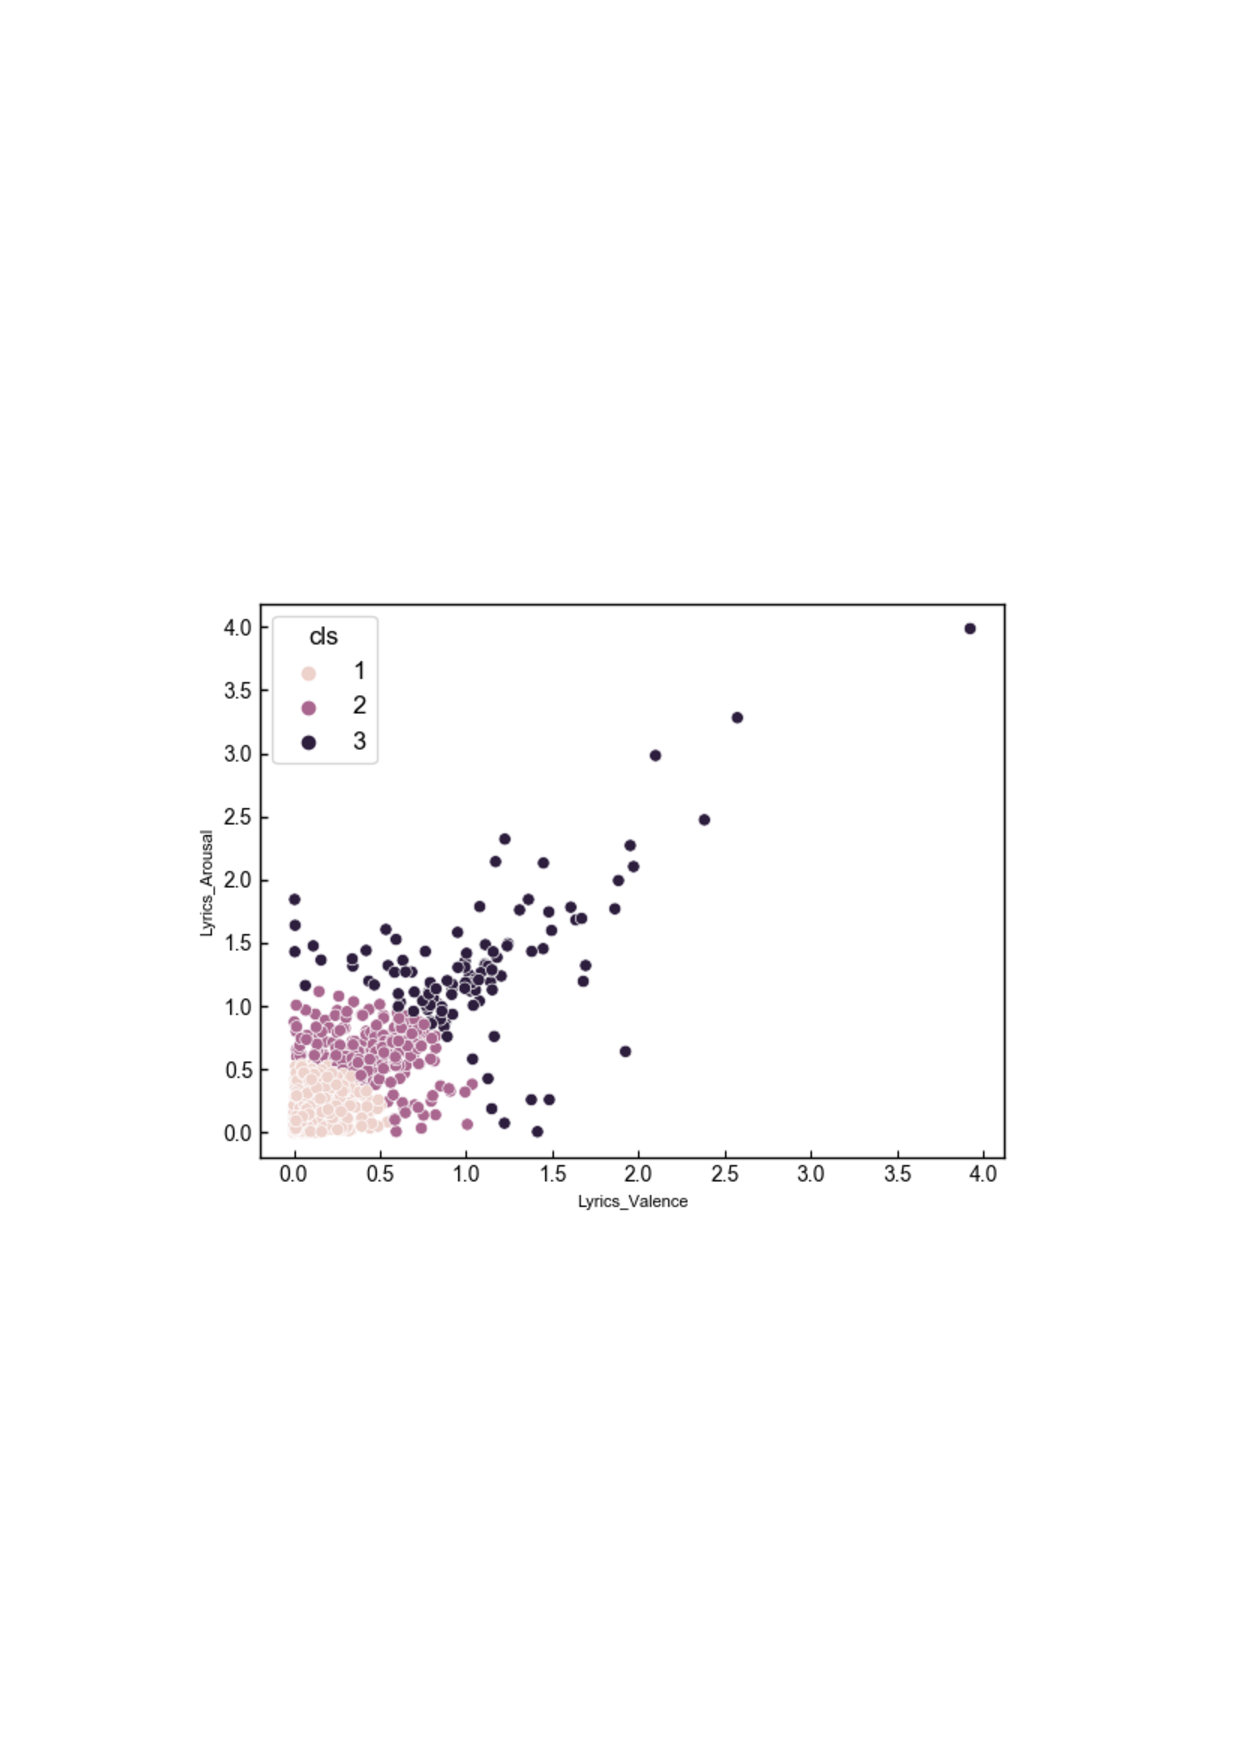
\includegraphics[width=14cm]{lyrics_A+V+.pdf}
  \vspace{-1mm}
  \caption{歌詞 A+V+平面}
  \label{fig:vkall}
  \vspace{5mm}
\end{figure}
第1象限にプロットされた楽曲は全部で1,424曲である.そのうちウォード法によって分割された曲数は第1グループが1015曲,第2グループが296曲,第3グループが112曲であった.
後述する実験に用いる楽曲の歌詞データはそれぞれのグループからランダムで1曲分選出する.
第1グループからはコブクロの「光の誓いが聴こえた日」,第2グループからは椎名林檎の「積み木遊び」,第3グループからはDREAM COME TRUEの「冬三昧にはまだ遠い」の3曲を選出した.
\newpage
第2象限のプロット図は図3.4である.
\begin{figure}[H]
  \centering
  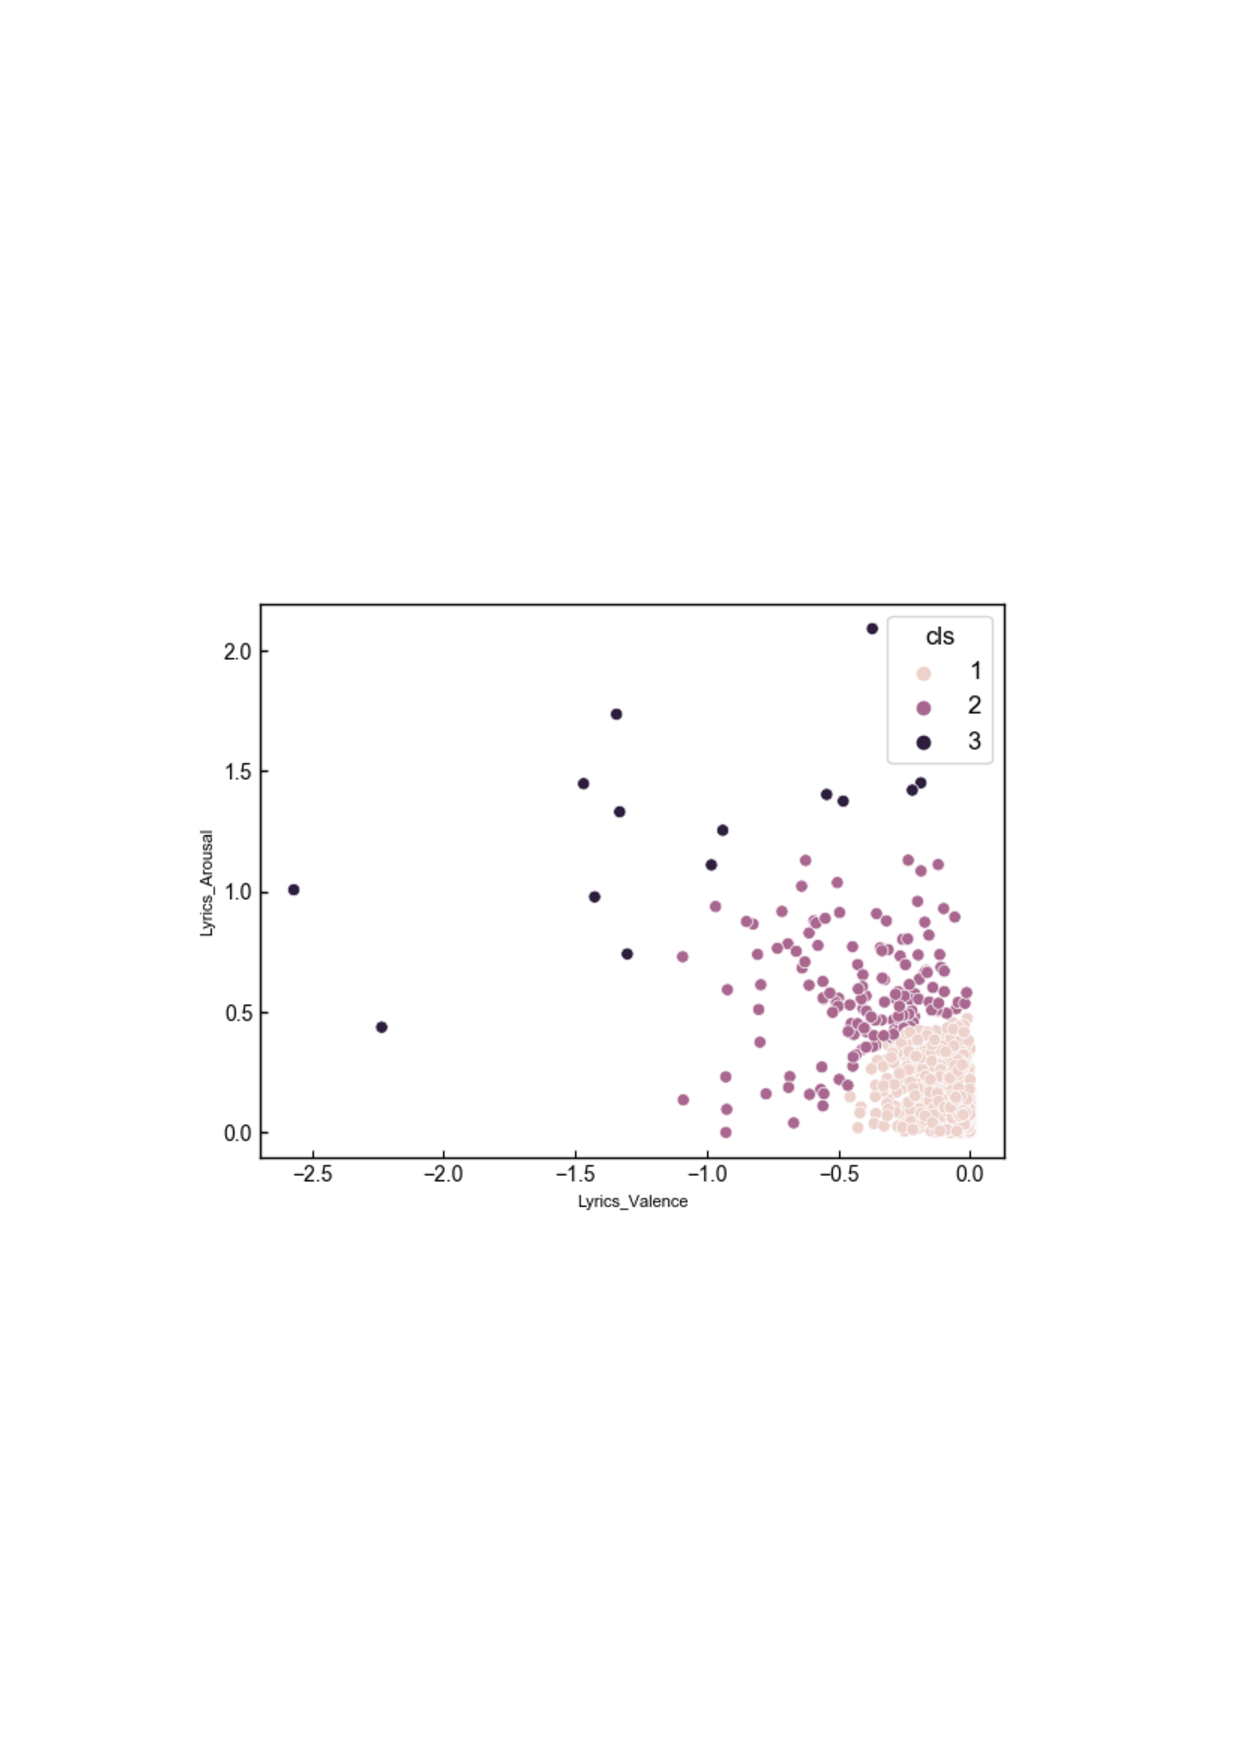
\includegraphics[width=14cm]{lyrics_A+V-.pdf}
  \vspace{-1mm}
  \caption{歌詞 A+V-平面}
  \label{fig:vkall}
  \vspace{5mm}
\end{figure}
第2象限にプロットされた楽曲は全部で887曲である.そのうちウォード法によって分割された曲数は第1グループが728曲,第2グループが145曲,第3グループが14曲であった.
後述する実験に用いる楽曲の歌詞データはそれぞれのグループからランダムで1曲分選出する.
第1グループからは,第2グループからはRADWIMPSの「透明人間18号」,第3グループからはB'zの「Da La Da Da」の3曲を選出した.
\newpage
第3象限のプロット図は図3.5である.
\begin{figure}[H]
  \centering
  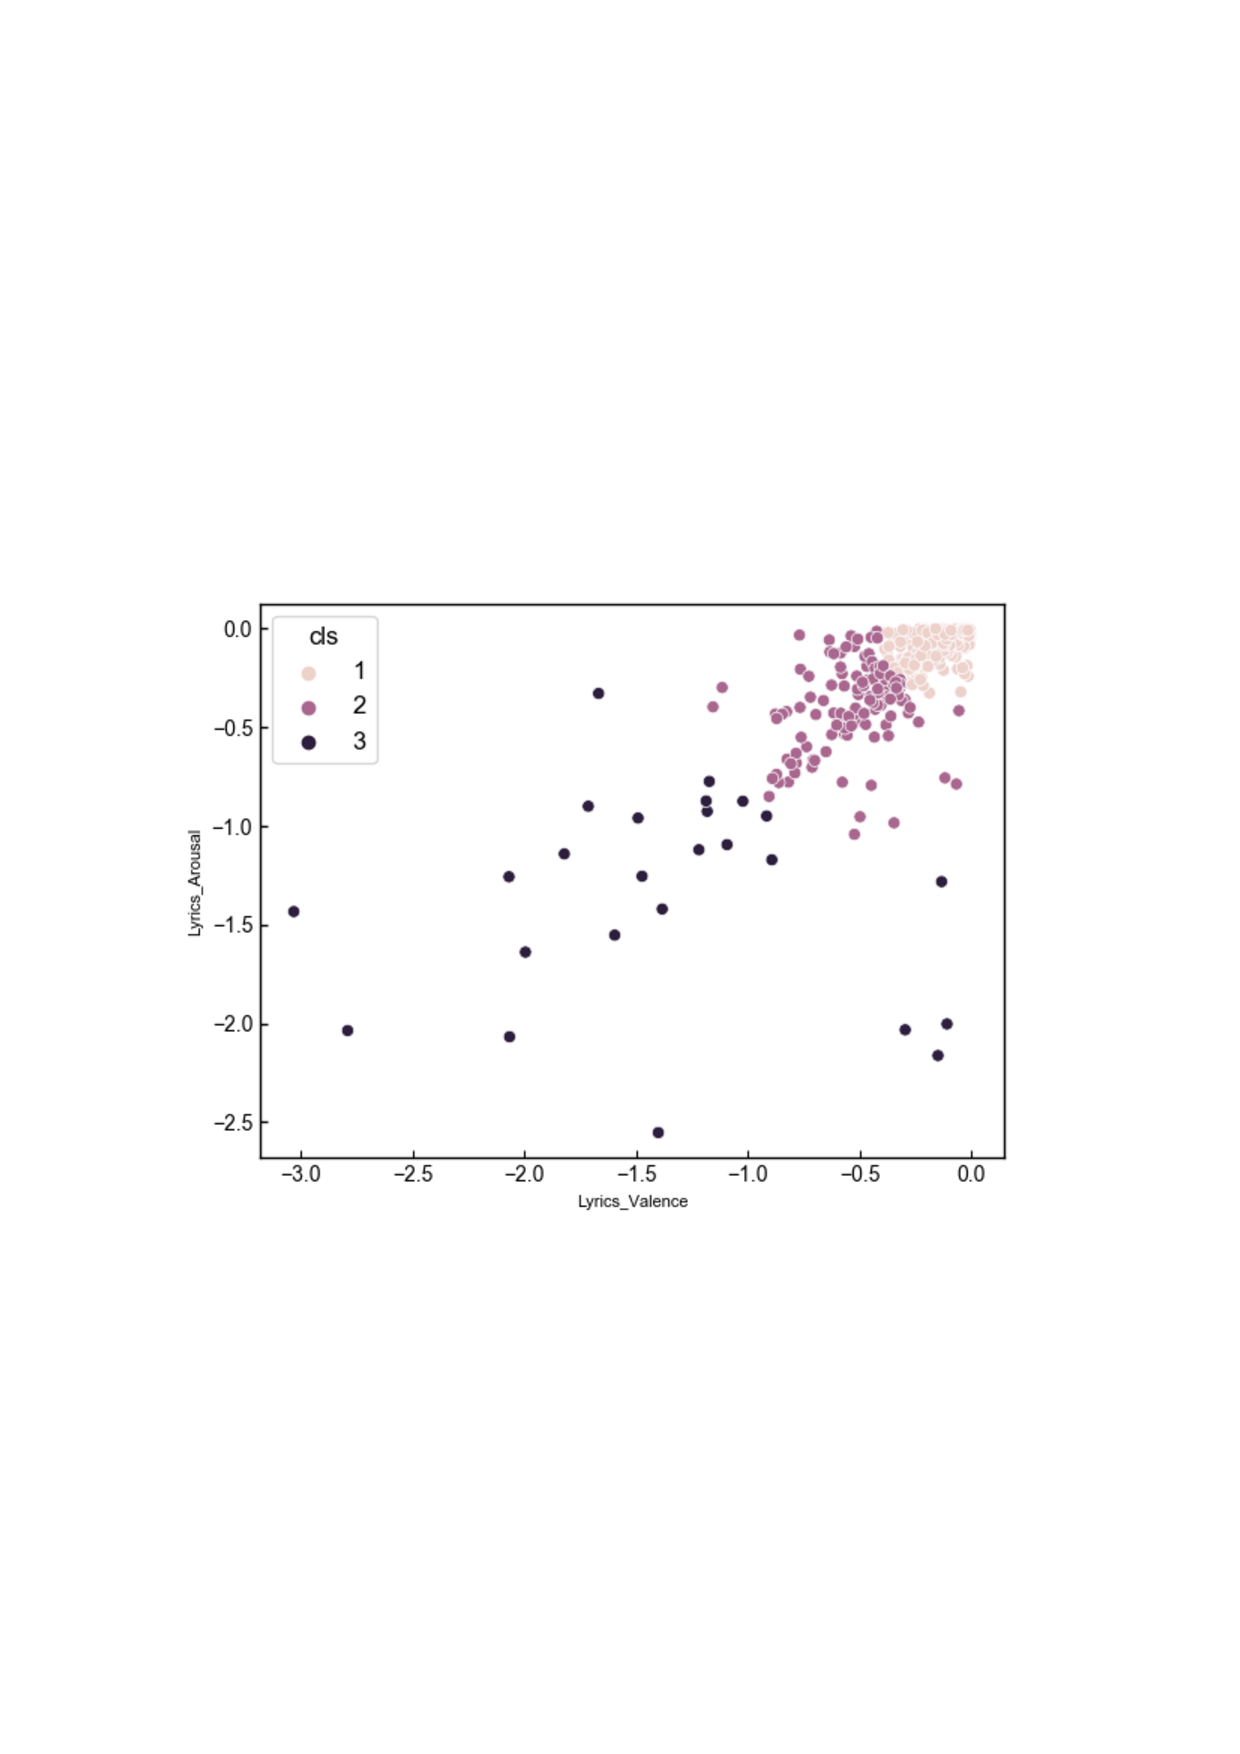
\includegraphics[width=14cm]{lyrics_A-V-.pdf}
  \vspace{-1mm}
  \caption{歌詞 A-V-平面}
  \label{fig:vkall}
  \vspace{5mm}
\end{figure}
第3象限にプロットされた楽曲は全部で388曲である.そのうちウォード法によって分割された曲数は第1グループが236曲,第2グループが127曲,第3グループが25曲であった.
後述する実験に用いる楽曲の歌詞データはそれぞれのグループからランダムで1曲分選出する.
第1グループからはEvery Little Thingの「Just be you」,第2グループからはコブクロの「コイン」,第3グループからはBUMP OF CHICKENの「分別奮闘記」の3曲を選出した.
\newpage
第4象限のプロット図は図3.6である.
\begin{figure}[H]
  \centering
  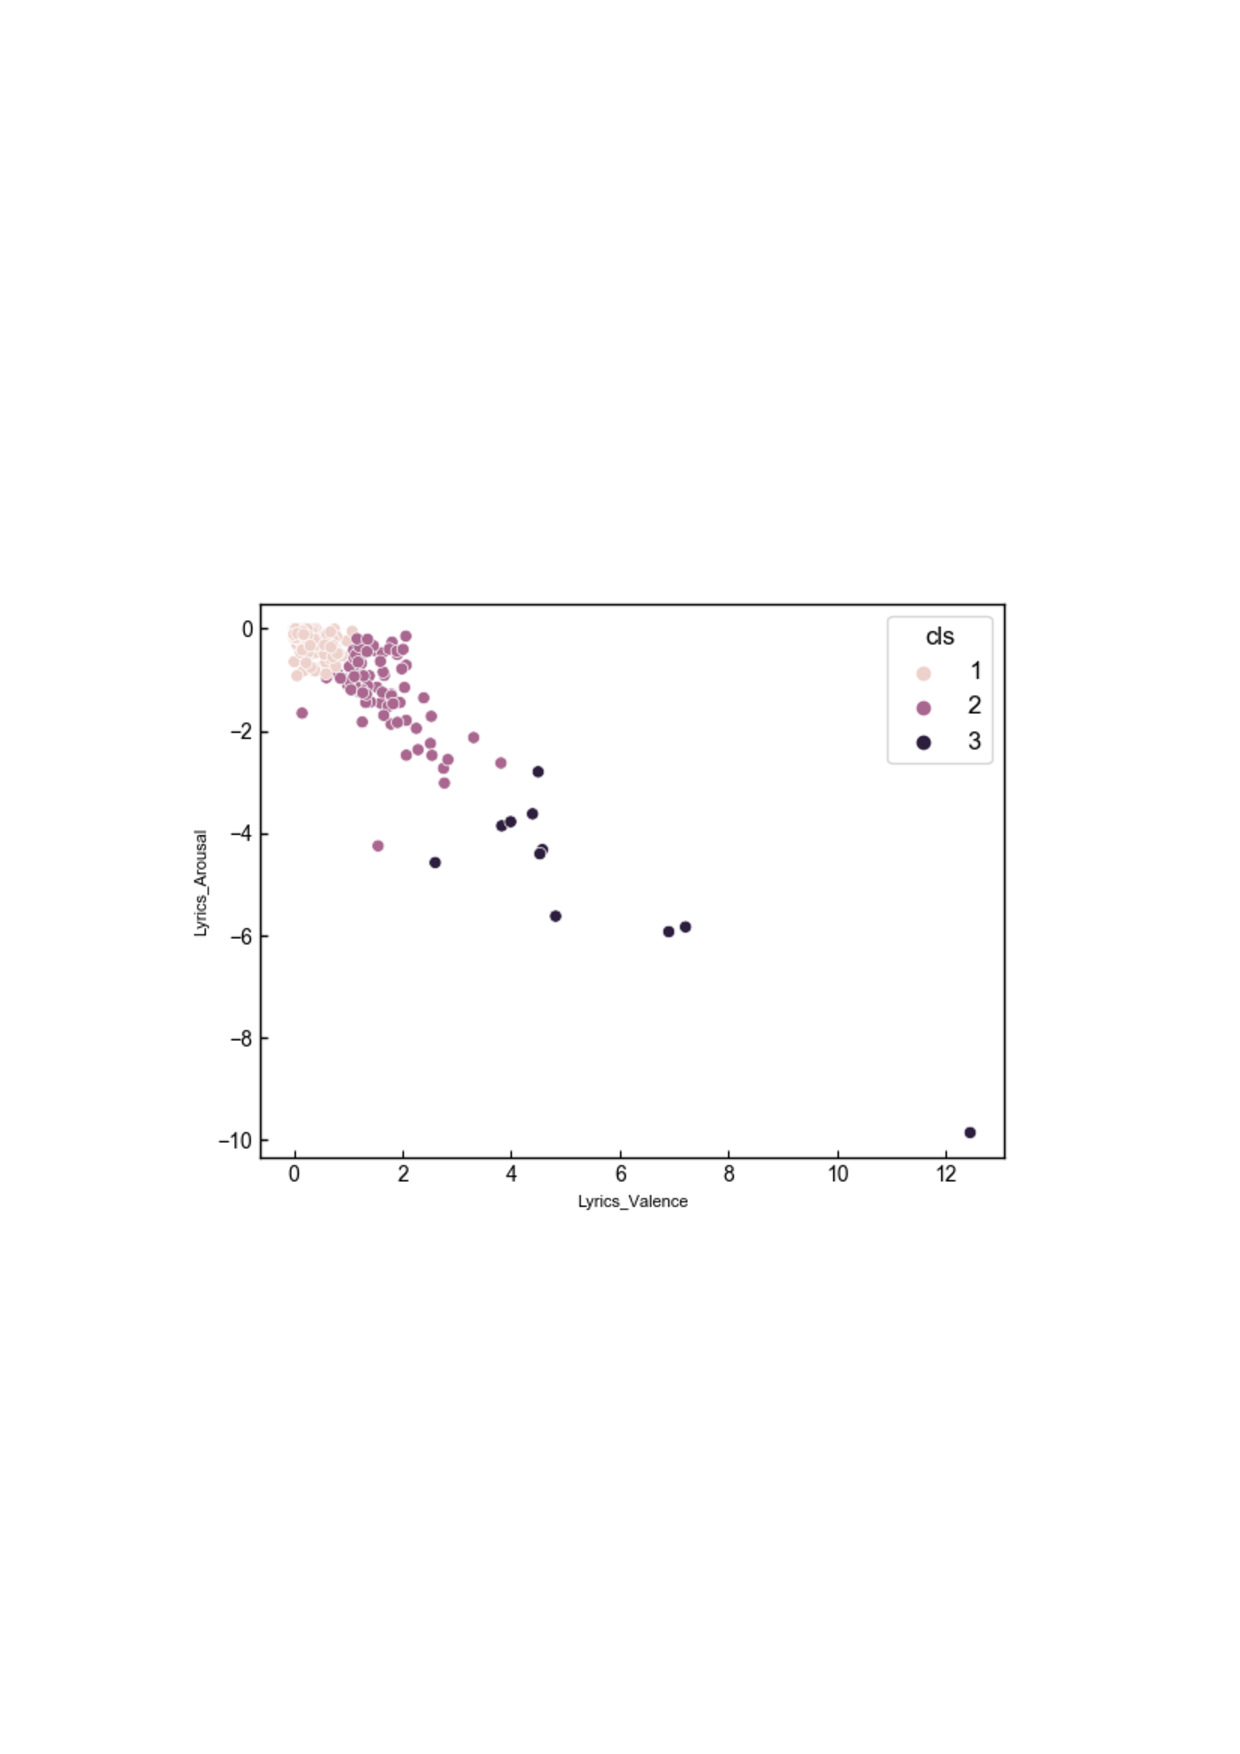
\includegraphics[width=14cm]{lyrics_A-V+.pdf}
  \vspace{-1mm}
  \caption{歌詞 A-V+平面}
  \label{fig:vkall}
  \vspace{5mm}
\end{figure}
第4象限にプロットされた楽曲は全部で302曲である.そのうちウォード法によって分割された曲数は第1グループが210曲,第2グループが81曲,第3グループが11曲であった.
後述する実験に用いる楽曲の歌詞データはそれぞれのグループからランダムで1曲分選出する.
第1グループからはUVERworldの「若さ故エンテレケイア」,第2グループからはあいみょんの「お互い様やん」,第3グループからはスピッツの「シロクマ」の3曲を選出した.
\newpage
\subsection{フレーズ}
歌詞に登場するフレーズをAV平面にプロットした.図3.7はAV平面に楽曲をプロットした図である.
\begin{figure}[H]
    \centering
    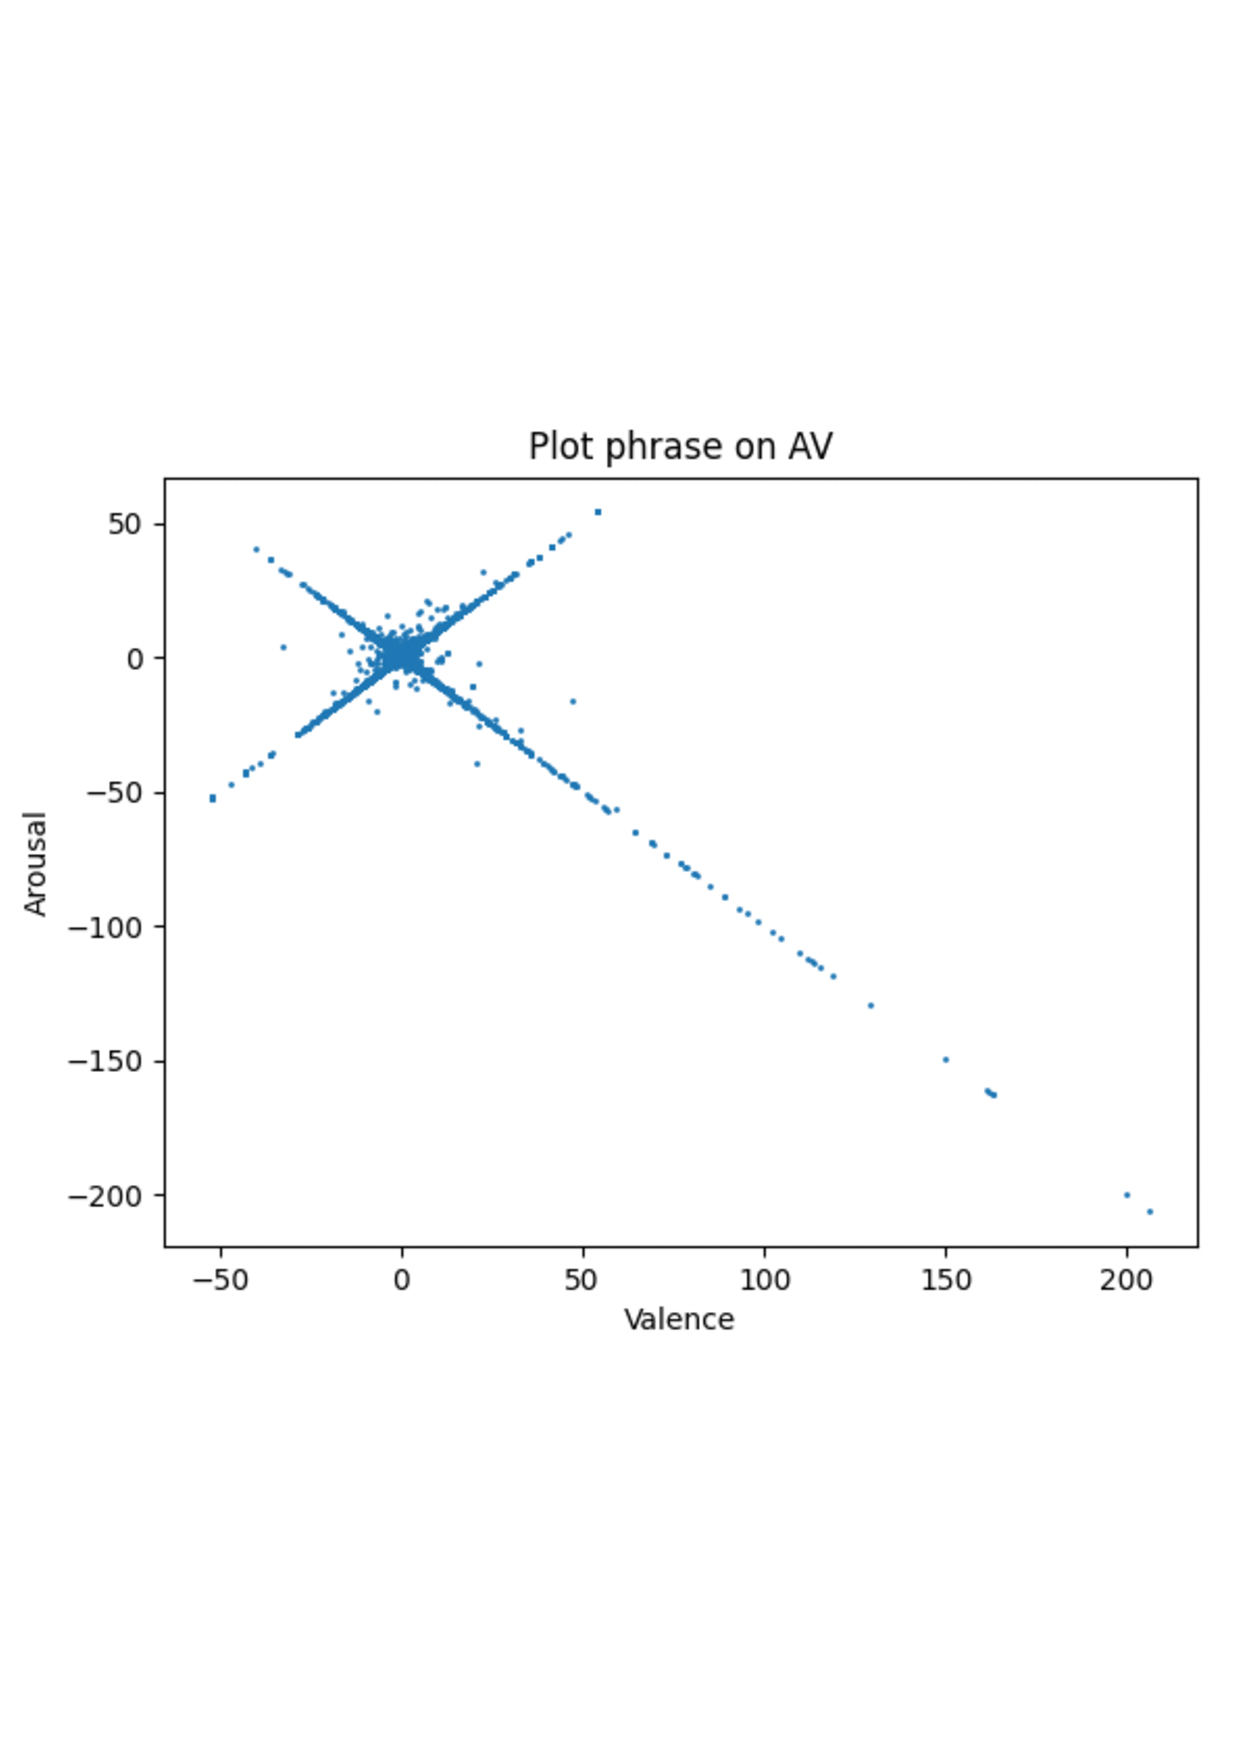
\includegraphics[width=12cm]{phrase_AV.pdf}
    \vspace{0mm}
    \caption{フレーズ AV平面}
    \label{fig:mms}
    \vspace{5mm}
\end{figure}
歌詞と同じく各印象ごとにフレーズを分類して,原点からの距離に基づいてward法でクラスタリングした.
\newpage
第1象限のプロット図は図3.8である
\begin{figure}[H]
    \centering
    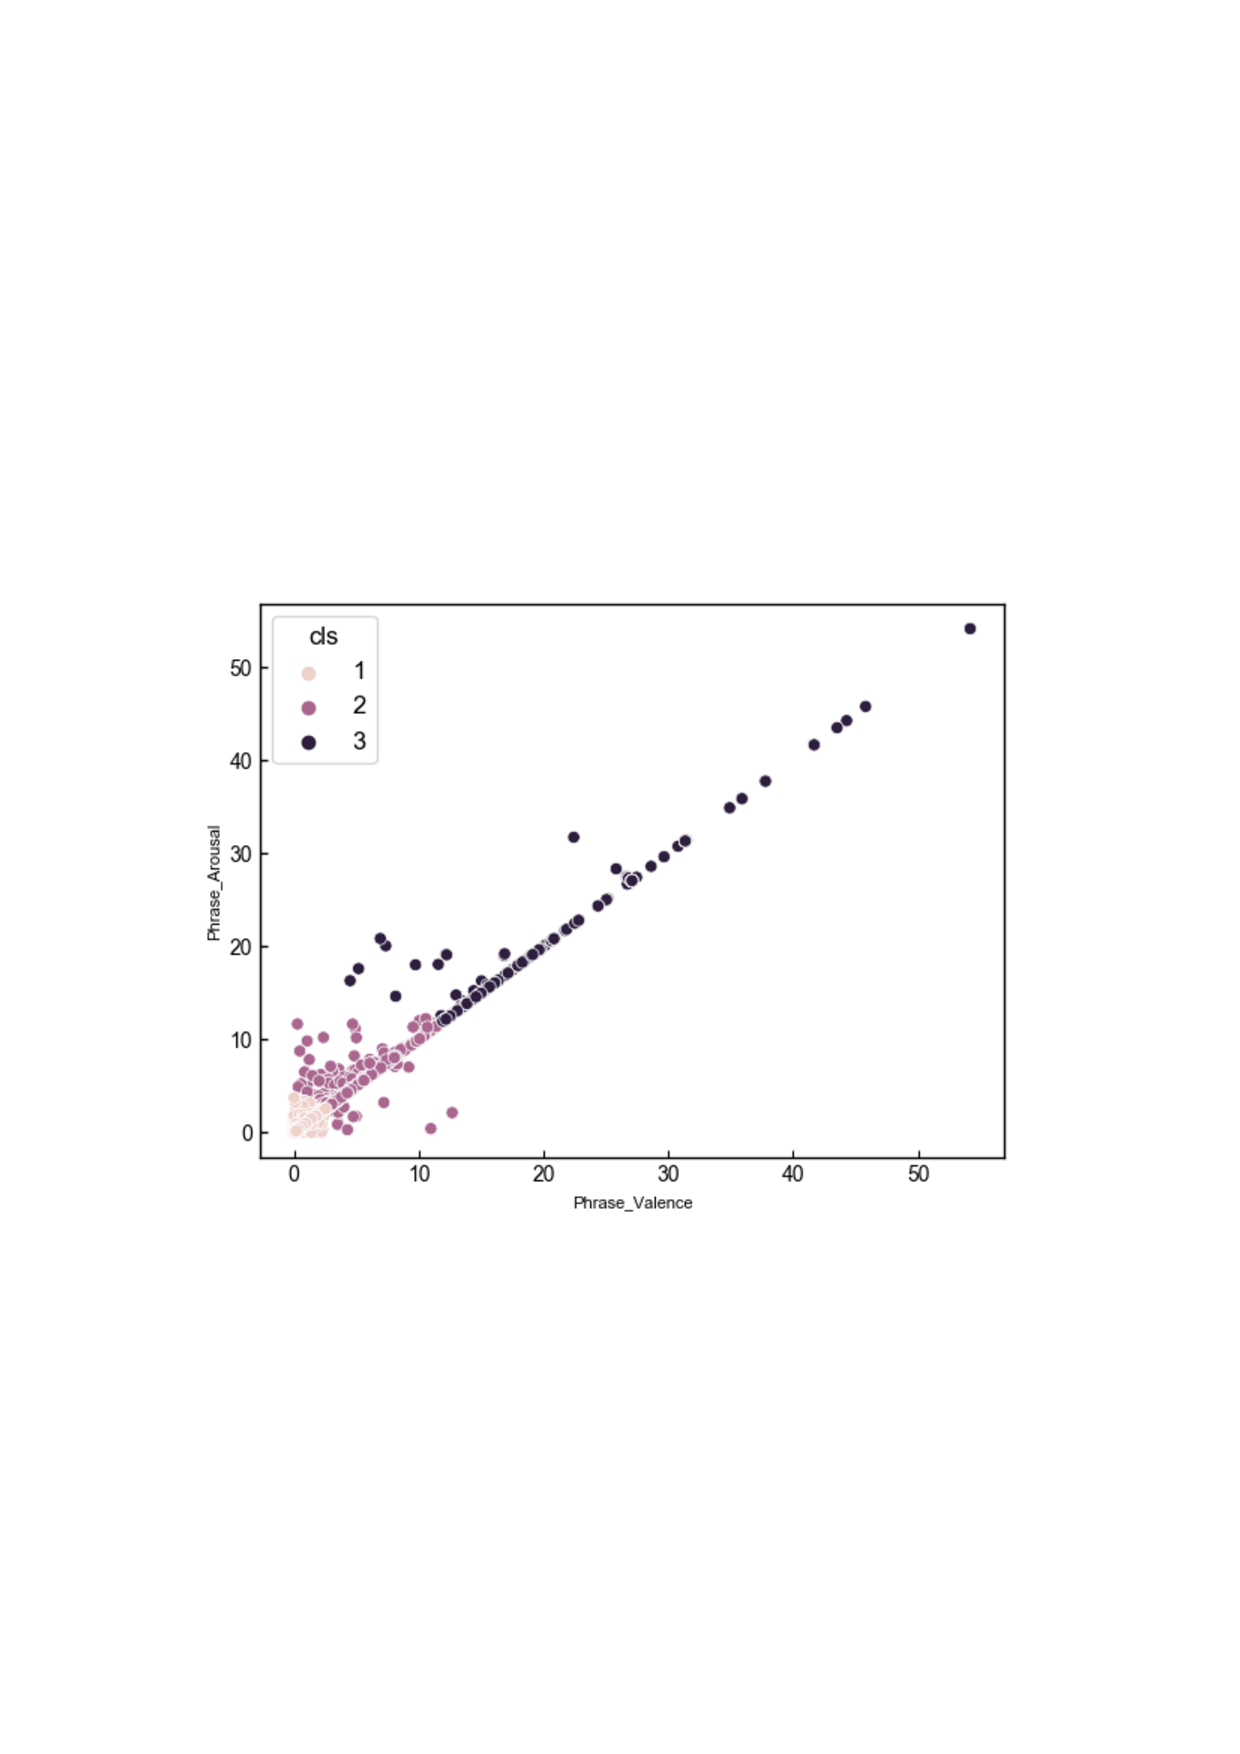
\includegraphics[width=14cm]{phrase_A+V+.pdf}
    \vspace{-1mm}
    \caption{フレーズ A+V+平面}
    \label{fig:mms}
    \vspace{5mm}
\end{figure}
第1象限にプロットされたフレーズは全部で35935句である.そのうちウォード法によって分割されたフレーズは第1グループが33,357句,第2グループが2,180句,第3グループが398句であった.
後述する実験に用いるフレーズのデータはそれぞれのグループからランダムで1句選出する.
第1グループからは「ひとりひとり違う世界みていくんだ」,第2グループからは「一石投じる生きる力」,第3グループからは「バタフライして」の3句を選出した.
\newpage
第2象限のプロット図は図3.9である.
\begin{figure}[H]
    \centering
    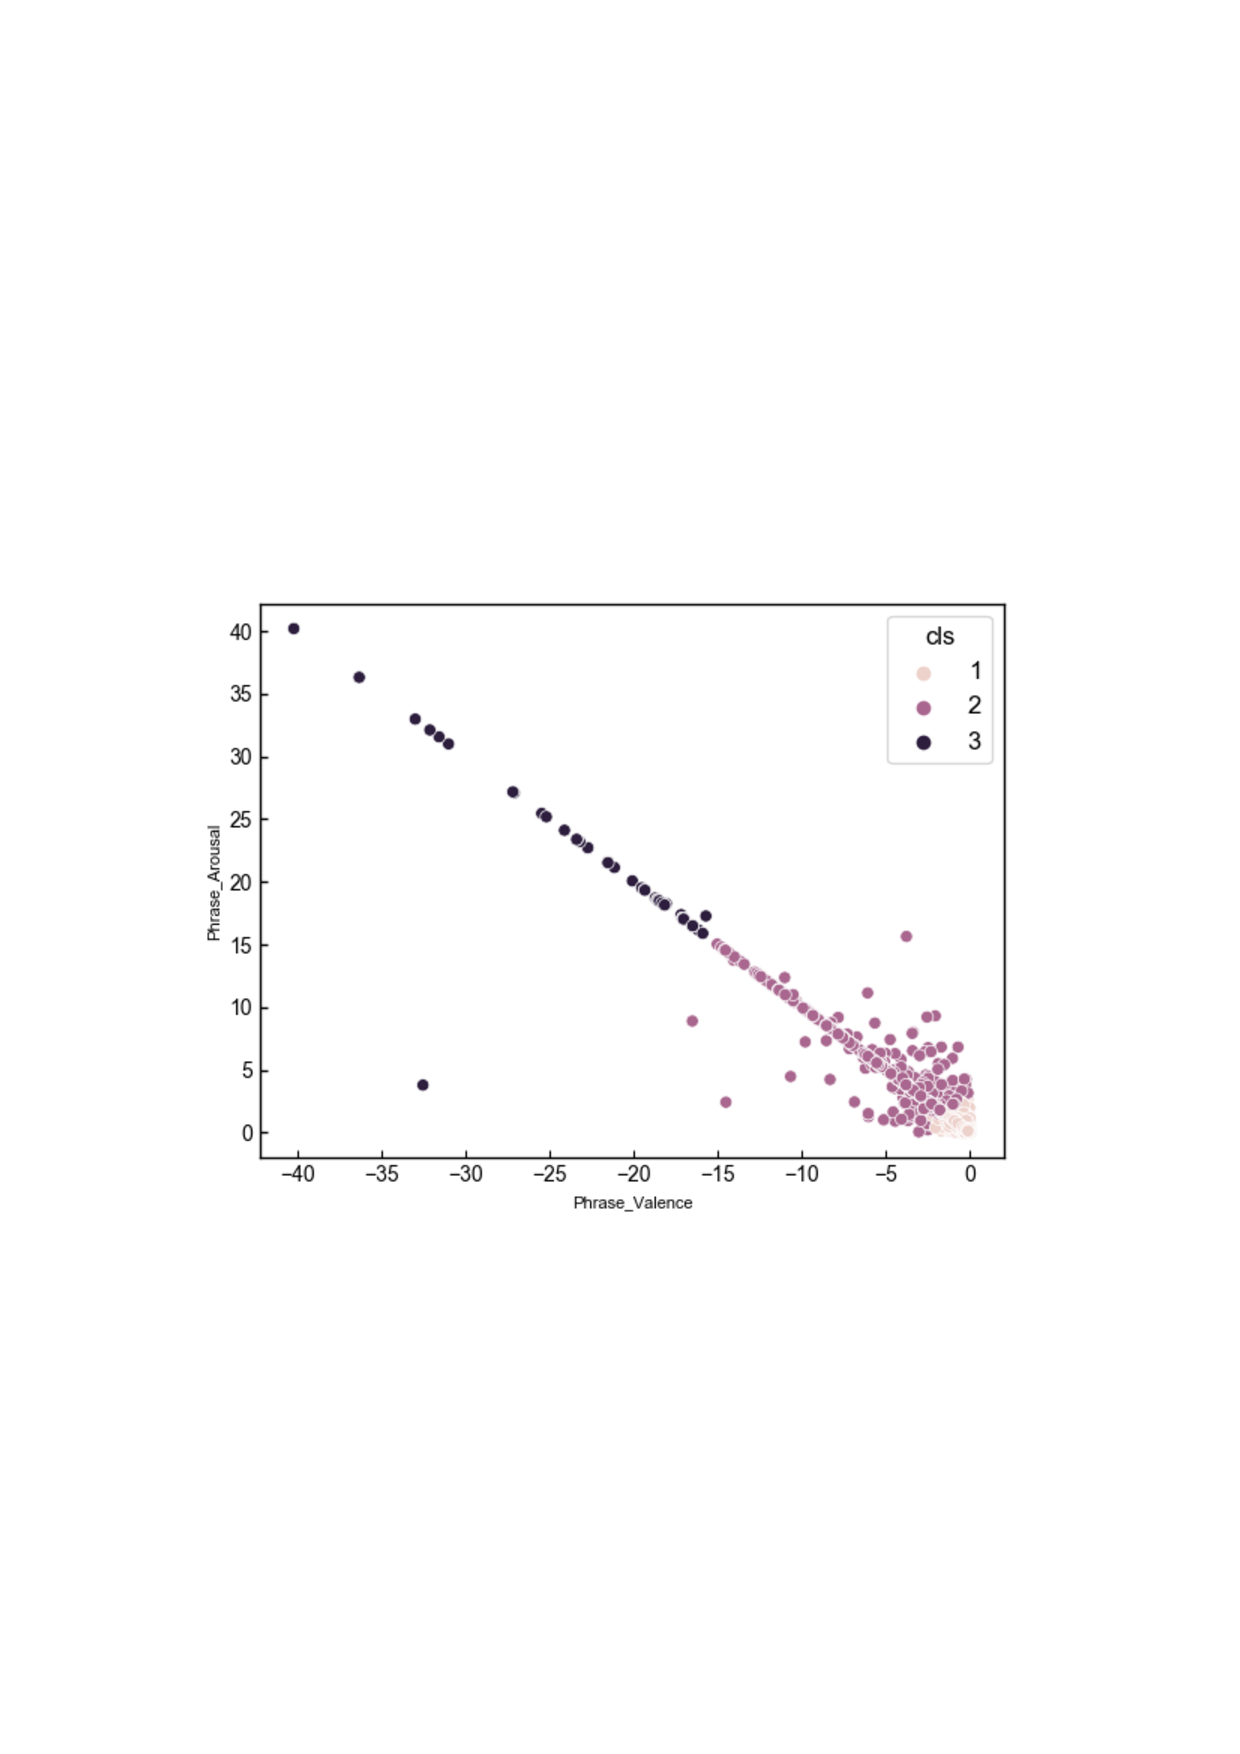
\includegraphics[width=14cm]{phrase_A+V-.pdf}
    \vspace{-1mm}
    \caption{フレーズ A+V-平面}
    \label{fig:mms}
    \vspace{5mm}
\end{figure}
第2象限にプロットされたフレーズは全部で27658句である.そのうちウォード法によって分割されたフレーズは第1グループが25,797句,第2グループが1,779句,第3グループが82句であった.
後述する実験に用いるフレーズのデータはそれぞれのグループからランダムで1句選出する.
第1グループからは「演じる意味はどこもブレたまま」,第2グループからは椎名林檎の「二つ並んだ影法師の手」,第3グループからはDREAM COME TRUEの「マイクホン争奪戦」の3句を選出した.
\newpage
第3象限のプロット図は図3.10である.
\begin{figure}[H]
    \centering
    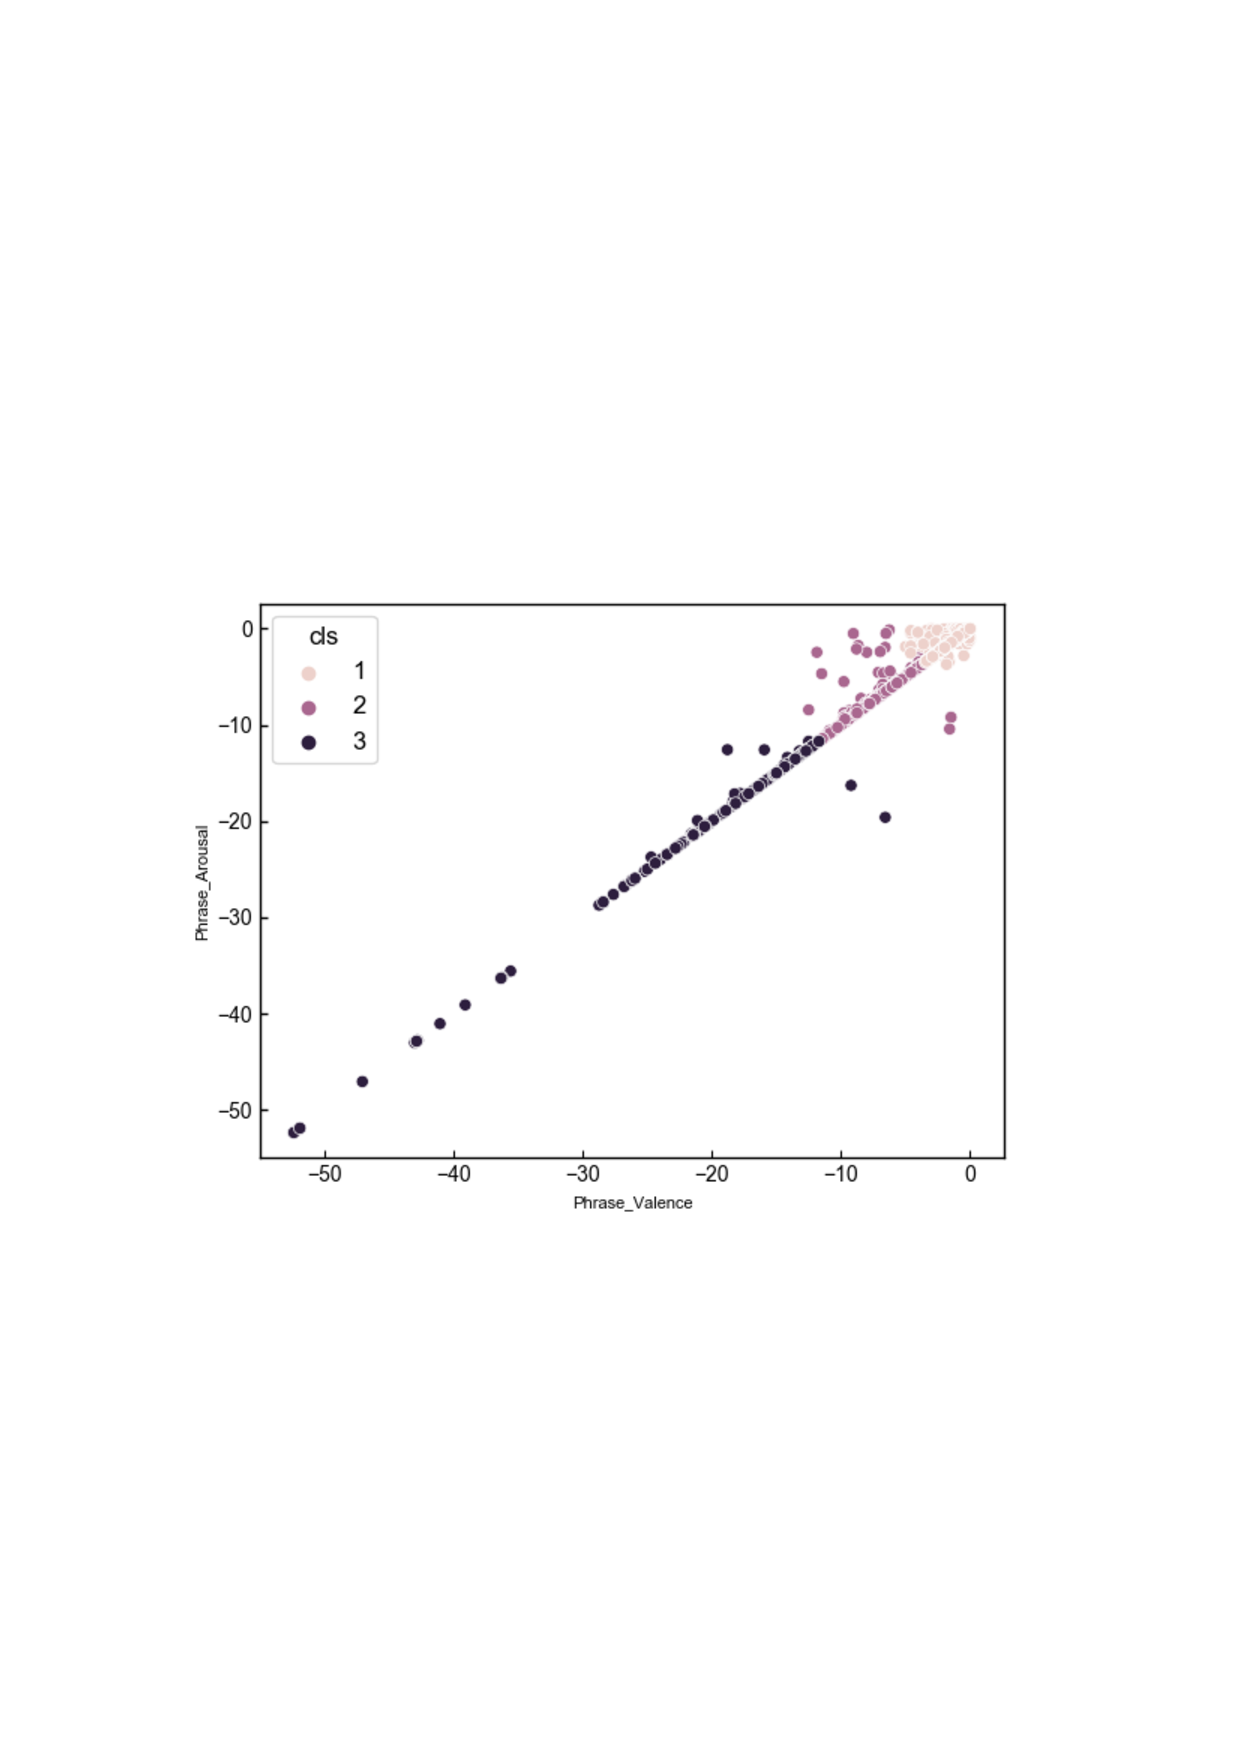
\includegraphics[width=14cm]{phrase_A-V-.pdf}
    \vspace{-1mm}
    \caption{フレーズ A-V-平面}
    \label{fig:mms}
    \vspace{5mm}
\end{figure}
第3象限にプロットされたフレーズは全部で14737句である.そのうちウォード法によって分割されたフレーズは第1グループが13,821句,第2グループが694句,第3グループが222句であった.
後述する実験に用いるフレーズのデータはそれぞれのグループからランダムで1句選出する.
第1グループからは「あたしを捨てたあなたは馬鹿で」,第2グループからは「あなたを苦しめたことでしょう」,第3グループからは「昨今のあなたは鼻につくわ」の3句を選出した.
\newpage
第4象限のプロット図は図3.11である.
\begin{figure}[H]
    \centering
    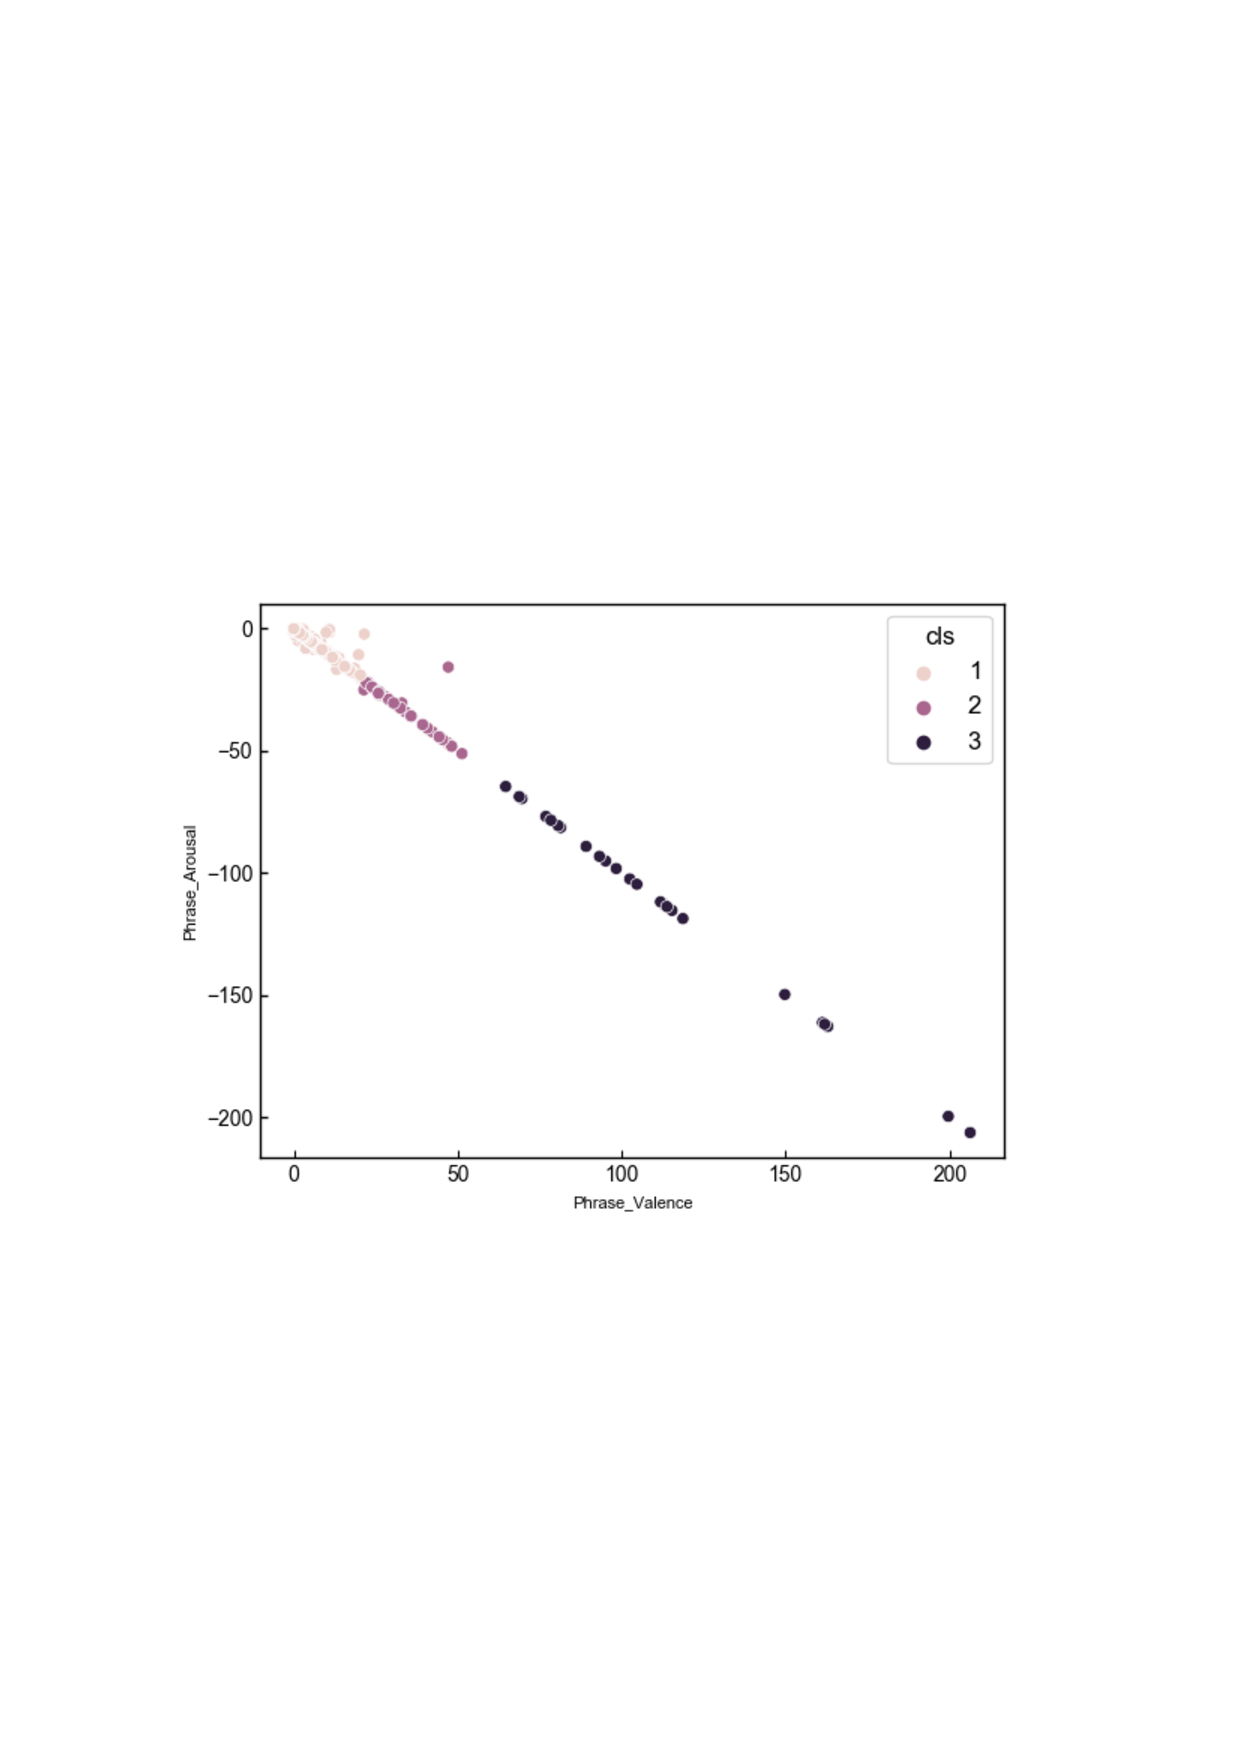
\includegraphics[width=14cm]{phrase_A-V+.pdf}
    \vspace{-1mm}
    \caption{フレーズ A-V+平面}
    \label{fig:mms}
    \vspace{5mm}
\end{figure}
第4象限にプロットされたフレーズは全部で60,000句以上である.第4象限にプロットされたフレーズ数は多かったので,重複削除をした後にランダムで30,000句を取り出した.そのうちウォード法によって分割されたフレーズは第1グループが29,907句,第2グループが64句,第3グループが29句であった.
後述する実験に用いるフレーズのデータはそれぞれのグループからランダムで1句選出する.
第1グループからは「浮かぶ月にやさしく響いては消えてった」,第2グループからは「染まる真っ赤なギロチン」,第3グループからは「しぶといトラウマも全部払おう」の3句を選出した.

%
\end{document}